\documentclass{standalone}
\usepackage[none]{hyphenat}
\usepackage{tikz}
\usetikzlibrary{positioning}
\usetikzlibrary{calc}
\usetikzlibrary{fit}
\usetikzlibrary{shapes}
\usetikzlibrary{arrows}
\usetikzlibrary{intersections}
\usetikzlibrary{shapes.geometric}
\usetikzlibrary{decorations.pathreplacing}

\begin{document}

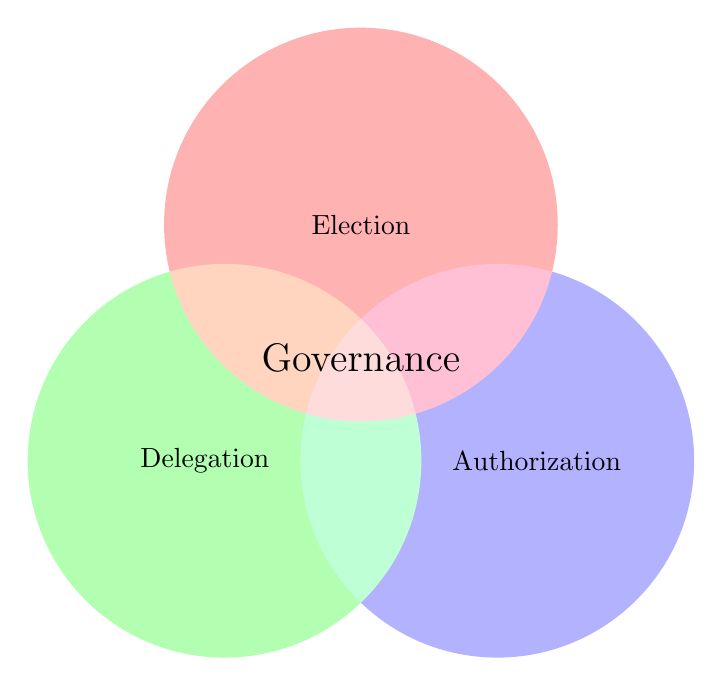
\begin{tikzpicture}[remember picture]
    \begin{scope}[blend group = soft light]
        \fill[red!30!white]   ( 90:2.0) circle (2.5);
        \fill[green!30!white] (210:2.0) circle (2.5);
        \fill[blue!30!white]  (330:2.0) circle (2.5);
    \end{scope}
    \node at (90:2.0)                   {Election};
    \node at ($(210:2.0) + (-0.25,0)$)  {Delegation};
    \node at ($(330:2.0) + ( 0.5,0)$)   {Authorization};
    \node at (90:0.3) [font=\Large]     {Governance};
\end{tikzpicture}

\end{document}
